
\section{Introduction}
\label{sec:intro}
Hyperspectral imaging (HSI) \cite{amigo2019hyperspectral} provides rich spectral information across hundreds of narrow bands, making it invaluable in domains like medical diagnostics \cite{fauvel2012advances}, remote sensing, and target detection \cite{uzair2013hyperspectral,technologies13050170}. However, a fundamental trade-off in optical systems means this rich spectral detail often comes at the cost of low spatial resolution, hampering downstream tasks such as classification \cite{he2017recent} and object tracking \cite{chen2021object}. To overcome this, Multispectral and Hyperspectral Image Fusion (MS/HS Fusion) has emerged as a key solution, aiming to reconstruct a high-resolution HSI by fusing a low-resolution HSI with a high-resolution multispectral image of the same scene.
In recent years, with the rapid development of deep learning, DL-based methods \cite{masi2016pansharpening,yang2017pannet,dian2018deep} have gradually become the mainstream for MS/HS Fusion. These methods can automatically learn complex nonlinear relationships, exhibiting immense potential in HSI fusion tasks.
\begin{figure}[!t]
    \centering
    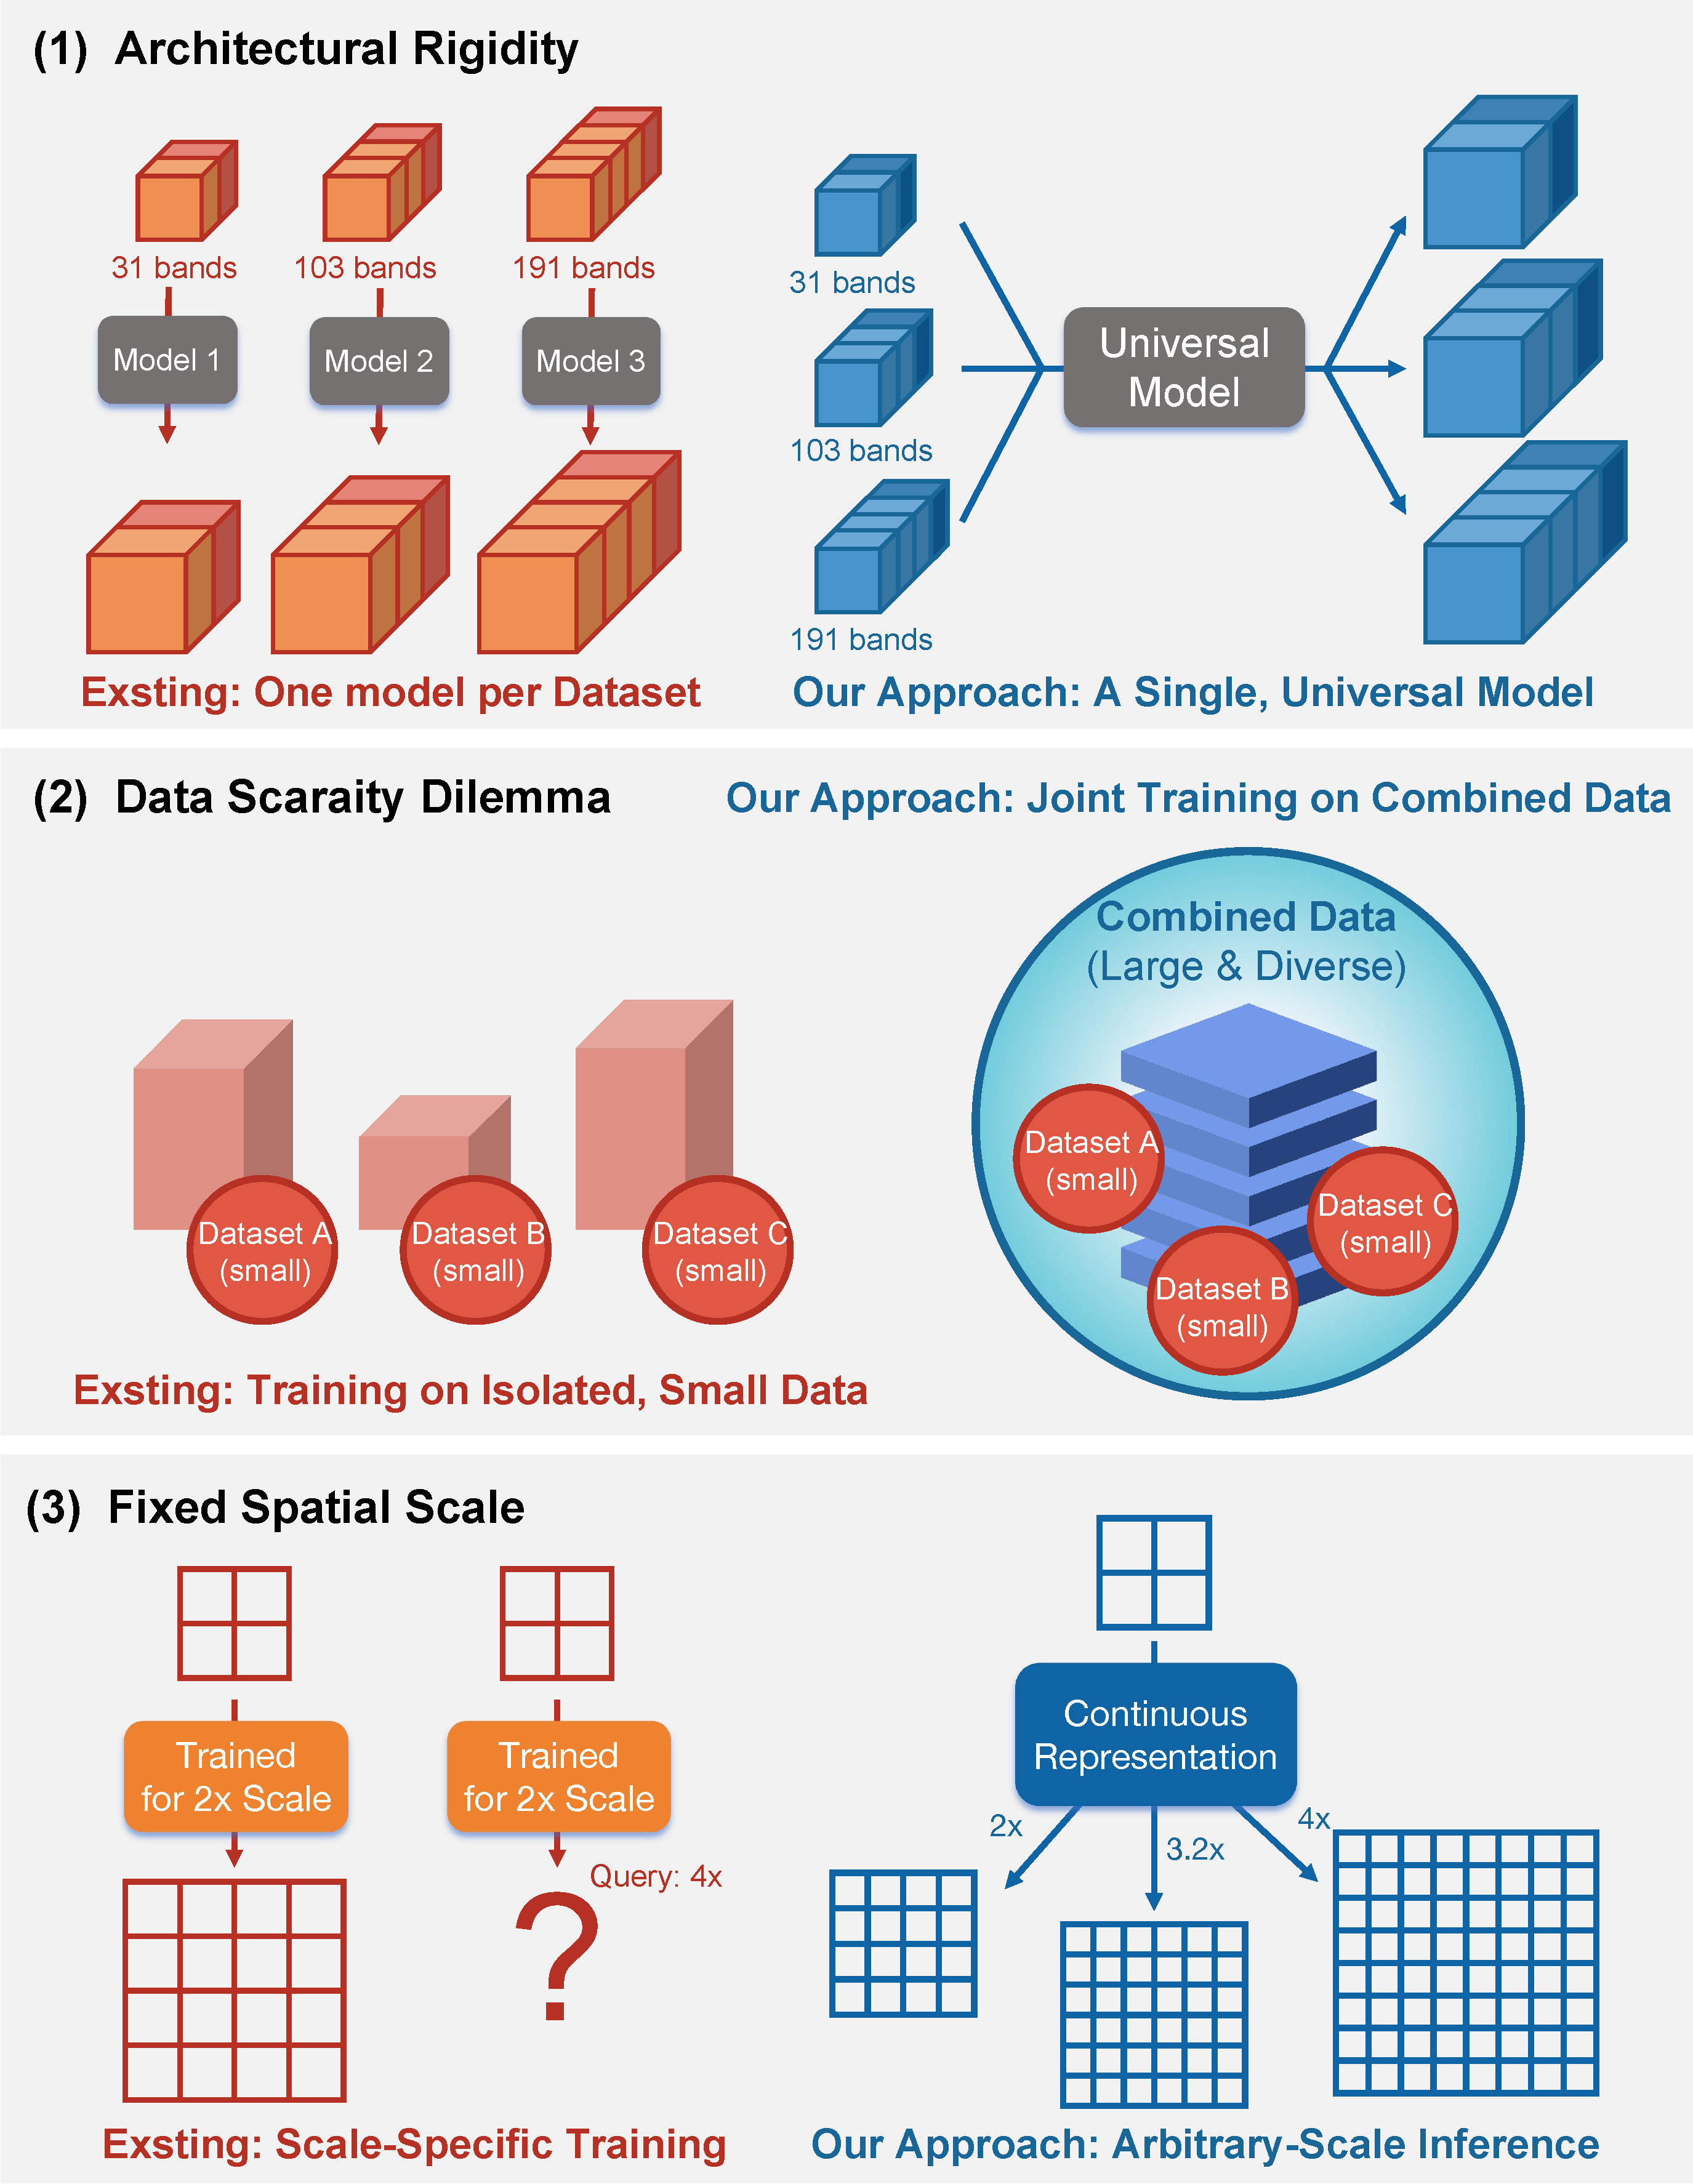
\includegraphics[width=\linewidth]{Figs/fig1.pdf}
    \caption{Existing paradigms \textit{v.s.} our universal approach for hyperspectral image fusion. Our method can suit different spectral bands joint training and can inference on arbitrary-scale fusion.}
    \label{fig:limitation}
    \vspace{-2em}
\end{figure}

Despite this significant progress, the real-world applicability of DL-based methods is hampered by the deep-rooted challenge of \textit{sensor diversity} \cite{hong2025hyperspectral}. Datasets captured by different sensors, such as AVIRIS (224 bands) or Pavia University (103 bands), vary drastically in their number of spectral bands, which exposes a fundamental lack of generality in current models. As illustrated in Fig.~\ref{fig:limitation}, this limitation manifests in three primary ways:
\textit{(1) Architectural Rigidity}: Most deep neural networks are designed with hard-coded channel dimensions, forcing researchers to either train independent models for each sensor~\cite{deng2023psrt, wu2025fully} or resort to costly fine-tuning~\cite{gonzalez2025multispectral}. Some even manually select band subsets~\cite{suryanarayana2025deep}, which sacrifices valuable spectral information.
\textit{(2) The Dilemma of Data Scarcity and Model Scale}: HSI datasets are typically small. Training on such isolated, small-scale data constrains model capacity and hinders the learning of generalizable features, leading to a high risk of overfitting~\cite{hoffmann2022training, yan2025hyperspectral}.
\textit{(3) Fixed Spatial Scaling Factor}: Current models~\cite{dengbidirectional, hu2022fusformer} are trained for a fixed integer upscaling factor (\textit{e.g.}, $4\times$, $8\times$). They learn a discrete grid-to-grid mapping, failing to handle the arbitrary or non-integer scales required in many applications.


To dismantle these barriers, we introduce SSA, a unified framework that addresses the above challenges through two technical innovations. To tackle spectral rigidity (1) and its impact on data scarcity (2), since hard-coded architectures prevent pooling data across sensors for large-scale training, we propose the Matryoshka Kernel (MK). Inspired by Matryoshka Representation Learning (MRL)~\cite{kusupati2022matryoshka}, MK allows a single model to process variable numbers of spectral bands, enabling joint training on heterogeneous datasets. Concurrently, to resolve spatial rigidity (3), we build our framework upon an Implicit Neural Representation (INR) backbone, which models signals as continuous functions and supports reconstruction at arbitrary (including non-integer) scaling factors.
In this work, we integrate these concepts into a cohesive MS/HS fusion model as a single unified framework. Our contributions are threefold:
\begin{itemize}
\item We introduce Matryoshka Kernels (MK), a novel architectural principle realized through adaptive convolution layers. This allows our model to natively process arbitrary numbers of spectral bands, enabling spectral-band agnosticism.
\item By building our framework upon an Implicit Neural Representation (INR), we replace discrete scaling with a continuous function, enabling reconstruction at arbitrary spatial scales.
\item Extensive experiments show that SSA achieves state-of-the-art performance while generalizing well to unseen sensors and scaling factors, substantially reducing the need for per-sensor retraining.
\end{itemize}
